\documentclass[10pt]{article}
\usepackage{tmlr}
\usepackage{amsmath,amssymb,booktabs,graphicx,array,microtype}
\usepackage[colorlinks=true,citecolor=blue,linkcolor=blue,urlcolor=blue]{hyperref}
\usepackage{url}
\newcommand{\ind}{\mathbf{1}}
\newcommand{\NComplete}{48}
\newcommand{\NDiscord}{39}
\newcommand{\NStateSuccess}{39}

\title{Auditing AI Agent Reliability:\\Policy Compliance and Failure-Monitor Evaluation}
\author{Anonymous authors}
\begin{document}
\maketitle
\begin{abstract}
A monitor's warning can be counted as a false alarm when final database state alone defines success. We audit how declared targets change negative classes and warning timing. Three separately analyzed cohorts cover 60 reserved retail and airline test IDs, with 227 completed conversations and 13 retained interrupted attempts. In the original cohort, all 39 state successes violate an explicit interaction constraint, and Gemini's first warning coincides with that violation in all 48 conversations. Additional monitor configurations do not necessarily share this timing. The final expansion supplies 49 interaction-clean state successes across 16 tasks; Gemini, DeepSeek and GPT-5.4 Mini alert on 2/49, 28/49 and 32/49, respectively. These are proxy-relative alert rates, not full-policy error rates. The exact interaction-rule baseline changes from 84/133 to 0/49 apparent false alarms solely through the negative-class definition. In 24 constructed cancellation pairs, every operation executes although half violate the executable eligibility rule. Both negative-class selection and a focused monitoring target change alert tradeoffs in configuration-dependent directions. We release matched public inputs, transparent baselines, missing-output accounting and executable analyses. The findings concern target alignment in a finite benchmark audit; they establish neither calibrated failure prediction nor comprehensive policy compliance.
\end{abstract}

\section{Introduction}
Tool-using agents combine language generation with actions that query or change an external environment, as illustrated by ReAct and Toolformer \citep{yao2023react,schick2023toolformer}.\footnote{LLM-based tools assisted with research planning, coding and analysis.} Their reliability must be evaluated along several dimensions that need not agree. An agent can reach an annotated database state while violating a conversational rule; it can follow a rule while disagreeing with an ambiguous reference outcome; and a monitor can flag either kind of problem. When these different targets are compressed into one success bit, the interpretation of a warning becomes unclear.

This concern is established in agent evaluation. Procedure-Aware Evaluation documents discrepancies between benchmark success and procedural integrity on $\tau$-bench \citep{cao2026procedure}. We do not claim to discover that successful outcomes can conceal procedural violations. Our focus is its consequence for \emph{monitor evaluation}: a warning that is correct for the monitor's stated target may be scored against a narrower negative class. That evaluation choice can change apparent false-alarm rates and the interpretation of warning timing.

The original $\tau$-bench evaluation compares the final database state with an annotated goal state \citep{yao2024tau}. This is an efficient outcome check, but it is not a universal oracle for every property in a natural-language policy. We use a pinned implementation from the maintained $\tau^2$-Bench repository \citep{barres2025tau2}, restricted to its retail and airline domains, and retain outcome matching as a separate, legitimate target. We do not evaluate its dual-control telecom setting. We deliberately compare different declared targets rather than assert that the benchmark's state label is intrinsically incorrect.

Our audit asks three questions. First, how often does state success coexist with a directly checkable interaction-contract violation in a held-out sample? Second, do monitor alerts anticipate that violation or merely identify it at the proposal boundary? Third, do superficial tool-name changes, explicit changes to the public policy, and a change in the monitor's requested target have distinguishable effects on its score? The third question is studied through controlled monitor inputs, separately from live actor experiments.

The evidence comprises three separately analyzed collection cohorts and a constructed eligibility experiment. The original factorial cohort establishes the target-alignment and timing audit; two later, prospectively frozen expansions add interaction-clean outcomes, repeated execution and additional monitor configurations. The constructed cases test a substantive cancellation rule with explicit simulator facts. This separation preserves the distinction between observed autonomous behavior and designed rule contrasts, and between an evaluation-label change and a change to the monitor prompt.

The study contributes an executable target-alignment audit, a matched record of actor/interface conditions, and controls that expose the source of an alert. It does not propose a new trained detector, estimate deployment-wide safety, or establish that a particular adaptation strategy is necessary. The contribution is a practical evaluation lesson: define the property to be monitored before treating successful benchmark episodes as negative examples.

\section{Targets, alerts and an accounting identity}
\label{sec:targets}
Let $x_{0:T}$ denote a recorded interaction, with an event index covering user messages, assistant proposals and tool results. Let $G=1$ when the native final-database check matches its reference and the conversation terminates normally. This definition is deliberately called \emph{state success}; nonempty natural-language assertions and broader semantic policy requirements are separate components.

Let $V=1$ when the record violates either of two explicit interaction constraints: an assistant message proposes more than one tool call, or an assistant message contains both tool calls and nonempty user-facing text. The domain policies state these constraints, and the native agent instruction also separates user messages from tool calls. A deterministic parser can therefore label this narrow property without a language-model judge. $V=0$ means only that these two violations were not observed. It does not establish that every policy was followed.

For a score $s_t$ at a generated assistant decision boundary, define $A_t=\ind[s_t\geq 0.5]$ and $A=\max_t A_t$. We keep this exploratory threshold fixed from development; it is not calibrated to a desired false-alarm rate. Two plausible negative classes give different quantities:
\begin{align}
 F_G &= \Pr(A=1\mid G=1),\\
 F_{G,\neg V} &= \Pr(A=1\mid G=1,V=0).
\end{align}
We call them \emph{apparent false-alarm rates relative to the named proxy target}. The second target adds only the measured interaction contract, not comprehensive policy review.

Let $q=\Pr(V=1\mid G=1)$. Where the relevant conditional populations have nonzero support, the law of total probability gives
\begin{equation}
 F_G=q\Pr(A=1\mid G=1,V=1)+(1-q)F_{G,\neg V}.
 \label{eq:decomposition}
\end{equation}
This is an accounting identity, not a new statistical estimator. The distinction between an intended construct and its operational measurement has a broader precedent in measurement-validity research \citep{jacobs2021measurement}; here we apply it to explicit monitor targets. It makes the target mismatch explicit: an exact contract detector with $A=V$ has $F_G=q$, although its false-alarm rate on contract-clean state successes is zero when that population exists. If every state success violates the contract, the second rate is undefined. Reporting a zero denominator as zero false alarms would conceal the lack of negative examples.

Timing needs the same care. Let $t_V$ be the first offending assistant proposal and $t_A$ the first alert. A monitor that receives that proposal and alerts at $t_A=t_V$ performs detection at the decision boundary. It has not demonstrated prediction before the violation became observable. This clock also prevents a post-tool observation from being credited with preventing an action already executed. We report before, at, after, and absent alerts separately; we do not infer the first irreversible task mistake from a terminal state label.

\section{Experimental protocol}
\label{sec:protocol}
\subsection{Development and held-out allocation}
Development used four upstream-training task IDs, two per domain. It produced 15 completed initial trajectories and one infrastructure interruption; a separately recorded new attempt later completed that cell. These data informed the audit and do not enter the held-out estimates. Forty development reference paths were also checked for equivalence under the initial interface wrapper. A released CPU-monitor reproduction is reported separately in Appendix~\ref{app:reproduction}.

For the original cohort, six upstream-test task IDs per domain were selected by a fixed SHA256 ordering before their model outputs were collected. The allocation crossed 12 tasks with two actors and two interface conditions, yielding 48 planned cells and one realization per cell. Tasks with an initial message history would be ineligible because that mapping was not implemented; no task was excluded by that rule. The task list, hypotheses, threshold, missingness policy and planned analysis were frozen locally. Execution amendments and output-truncation handling are separately recorded; they do not change model settings or remove selected task cells. This is a prospective local protocol record, not an externally registered preregistration.

Task IDs are disjoint from development. They are not claimed to be disjoint task families: the domains reuse workflows and databases. We group exact reference-operation sequences for a sensitivity analysis and disclose that this is only a coarse family proxy. The evaluation therefore supports a descriptive audit of this sample, not an estimate for all customer-service deployments.

\subsection{Actors, interfaces and execution}
The benchmark revision is \texttt{b7ea9074c1cba482b30687fecdb5c8425fd6f619} from the maintained Sierra Research repository. We use its native retail and airline tools, task data, agent prompt and customer-simulator orchestration. The acting models are Claude Sonnet 5 and DeepSeek V4.1 Flash; the customer simulator is fixed to Claude Sonnet 5. Gateway model IDs, provider allowlists, token limits and reasoning settings are in Appendix~\ref{app:configuration}. These are hosted aliases, not immutable weight snapshots. Sampling is not seed-pinned.

The original interface uses native tool names. The renamed interface adds \texttt{service\_} to each tool name except \texttt{calculate}, whose ordinary-language use in documentation would introduce an additional wording change. Visible references are updated, arguments and execution remain unchanged, and an evaluator-only inverse map restores canonical names. Invalid legacy names remain invalid. All 12 selected reference paths were checked for equal tool responses, errors and intermediate database states before paid collection. This is an executable interface change, unlike a change applied only to stored monitor inputs.

Each original-cohort conversation is limited to 60 orchestration steps; later cohorts use separately declared limits. Infrastructure interruptions are retained separately from bounded task outcomes. A transport retries selected transient HTTP errors at most twice after the initial attempt, preserves each attempt, and keeps the model/provider route fixed. No trajectory is silently replaced. Retail and airline collection use isolated processes sharing a locked study budget; this scheduling-only amendment was recorded before the assigned airline cells ran. Actor and interface order alternates within the fixed allocation.

The interface experiment pairs tasks, not stochastic conversations. The user simulator can respond differently across conditions, so an observed difference combines actor and dialogue variation. We do not interpret a one-run paired difference as an isolated effect of naming on a monitor.

\subsection{Monitor inputs and baselines}
The original language-model monitor is Gemini 3.8 Flash with a fixed prompt asking about incorrect task outcomes, unfulfilled requests or policy violations. It receives the current public policy, current tool schemas, and the conversation prefix through the current assistant proposal. It does not receive private user instructions, reference actions, final database state, future messages or the eventual trajectory length. Each input has a stored hash, and tests verify that modifying hidden outcomes or future turns does not change an earlier input.

We request a score at every model-generated assistant decision and retain invalid outputs as missing. Proposed tool calls are visible, but their results are not. Earlier tool errors are visible only after their responses arrive. Four transparent baselines share this observation clock: never alert; alert after an observed tool error; alert on a third identical proposed call; and alert on an explicit interaction-contract violation. Recovered tool errors and repeated calls are heuristic warning signals, not ground-truth task failures. The contract baseline is exact for $V$ by construction, which is its intended role as a diagnostic control.

\subsection{Controlled monitor-input checks}
An initial development diagnostic holds eight original-interface trajectories fixed. For each, it takes the first generated assistant decision and first multi-call proposal, giving 16 prefixes from four task IDs. Each prefix is scored twice unchanged and once after a reversible tool-name/documentation transformation. The 48 calls rotate arm order. Argument constraints, conversation length and observed behavior are preserved. No label or state transition is changed, and this experiment is not described as a new live actor trajectory.

An exploratory held-out follow-up is specified before its monitor calls. It selects one actor/interface cell per task by a fixed hash and uses its first batch proposal, if present. Cells without a batch, or with an earlier mixed text/tool violation that would survive the intervention, remain explicitly ineligible. Three arms repeat the strict-policy input, change only the public sentence governing batch calls to permit them in listed order, or retain the strict policy but ask an outcome-focused monitoring question. The latter excludes interaction-format violations alone as evidence of an incorrect final database state. These interventions test score interpretation at identical proposed actions. They are not live actor interventions or evidence of improved task completion.

\subsection{Analysis and uncertainty}
We report raw counts by domain, actor and interface. State/contract discordance is estimated as $\sum GV/\sum G$. Apparent alert rates are evaluated against both named negative classes without calling either comprehensive ground truth. First-alert timing uses the explicit contract onset, not an inferred task-failure onset.

Invalid or truncated structured responses are missing scores, never negative predictions. When a valid alert precedes every missing prefix in an episode, both its any-alert status and first-alert time are still identified. We verify that condition before including such an episode in the alert analysis. One same-setting recovery of a truncated response was attempted and separately retained; no token-cap increase or score imputation was used.

Bootstrap resampling provides an empirical uncertainty estimate \citep{efron1979bootstrap}. Prior work on stochastic agent evaluation highlights the sensitivity of conclusions to few runs and reporting choices \citep{henderson2018matters,agarwal2021precipice}. Our uncertainty analysis uses 5,000 bootstrap replicates, stratified by domain and resampling whole task IDs with all actor/interface cells together. A second analysis resamples reference-operation-sequence groups. These intervals describe variability across a small finite sample; they are not deployment guarantees. Undefined replicate denominators are counted, and degenerate intervals are not evidence of certainty. No prefix is treated as an independent task, no hypothesis is selected by its $p$-value, and no held-out data are used to tune a threshold or train a detector.

\section{Results}
\label{sec:results}
All 48 planned cells completed, with 511 of 514 generated assistant decisions scored. 3 prefixes lack valid structured output at the fixed token cap; these are retained as missing. In every affected conversation an observed alert precedes the missing prefix, so the episode-level any-alert decision and first-alert time remain identified. There are 12 task IDs and 11 distinct reference-operation-sequence groups. The native database check with normal termination marks 39 conversations as state successes; 48 conversations contain an explicit interaction-contract violation. Both labels hold in 39/39 state successes (100.0\%; the domain-stratified task bootstrap interval is [100.0\%, 100.0\%]. The operation-sequence-group sensitivity interval is [100.0\%, 100.0\%]. Both intervals are degenerate because every sampled state success violates the contract; they do not establish a population violation probability of one. Neither calculation had an undefined denominator (0 and 0 of 5,000 replicates, respectively). Table~\ref{tab:cohort} and Figure~\ref{fig:matrix} preserve the individual strata and task cells.

Against state success alone, the language-model monitor alerts on 39/39 negatives (100.0\%); the exact contract detector alerts on 39/39 (100.0\%). Adding the measured contract leaves 0 negative conversations. Table~\ref{tab:rates} reports the resulting denominators explicitly. This comparison changes the reference target while keeping the recorded alerts fixed; it is not a performance gain from retraining.

First alerts occur before the first contract violation in 0 conversations, at it in 48, and after it in 0. There are 0 violating conversations with no alert and 0 conversations without an observed contract violation. Figure~\ref{fig:timing} uses message-event indices rather than wall-clock latency. Coincidence with the first offending proposal is evidence of boundary detection, not advance warning of an unobserved failure. The deterministic contract baseline detects exactly the measured property by construction; its inclusion diagnoses target alignment rather than establishing a general-purpose monitor.


\begin{table}[t]
\centering\small
\caption{Held-out counts by domain, actor and interface. State success means database matching with normal termination. The contract column covers only the two explicit interaction constraints.}
\label{tab:cohort}
\begin{tabular}{lllrrrr}
\toprule
Domain & Actor & Interface & $n$ & $G=1$ & $V=1$ & $G=1,V=1$\\
\midrule
Retail & Sonnet & baseline & 6 & 5 & 6 & 5\\
Retail & Sonnet & rename & 6 & 5 & 6 & 5\\
Retail & DeepSeek & baseline & 6 & 5 & 6 & 5\\
Retail & DeepSeek & rename & 6 & 4 & 6 & 4\\
Airline & Sonnet & baseline & 6 & 4 & 6 & 4\\
Airline & Sonnet & rename & 6 & 5 & 6 & 5\\
Airline & DeepSeek & baseline & 6 & 5 & 6 & 5\\
Airline & DeepSeek & rename & 6 & 6 & 6 & 6\\
\bottomrule
\end{tabular}


\end{table}

\begin{figure}[t]
\centering
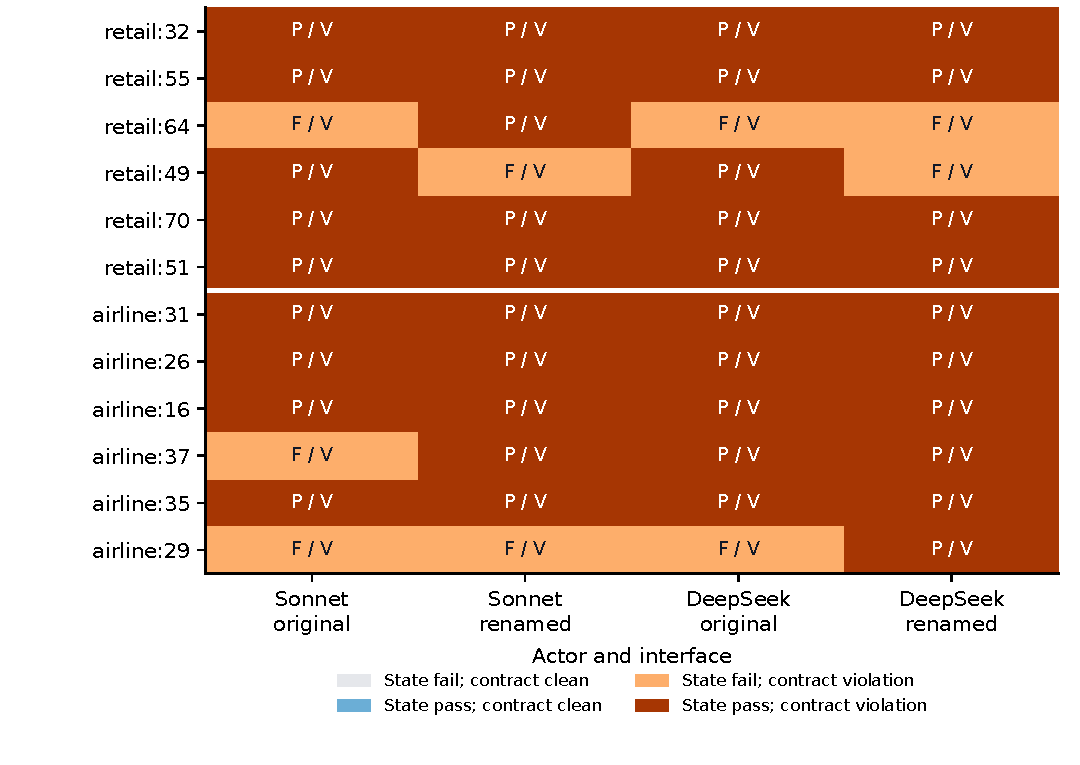
\includegraphics[width=0.96\linewidth]{figures/label_matrix.pdf}
\caption{State and interaction-contract outcomes for every held-out cell. Task rows, rather than individual decisions, are the sampling units. Passing one check does not imply passing the other.}
\label{fig:matrix}
\end{figure}

\begin{table}[t]
\centering\small
\caption{The original Gemini decisions evaluated against two declared negative classes. Entries are alerting episodes / negative episodes. ``Undefined'' means no eligible negative examples, not zero false alarms. These are proxy-relative rates, not independently adjudicated full-policy error rates.}
\label{tab:rates}
\begin{tabular}{lll}
\toprule
Monitor & State success $G=1$ & State success and $V=0$\\
\midrule
Never alert & 0/39 (0.0\%) & Undefined (0 negatives)\\
Observed tool error & 4/39 (10.3\%) & Undefined (0 negatives)\\
Repeated identical call & 0/39 (0.0\%) & Undefined (0 negatives)\\
Exact contract & 39/39 (100.0\%) & Undefined (0 negatives)\\
Language-model monitor & 39/39 (100.0\%) & Undefined (0 negatives)\\
\bottomrule
\end{tabular}


\end{table}

\begin{figure}[t]
\centering
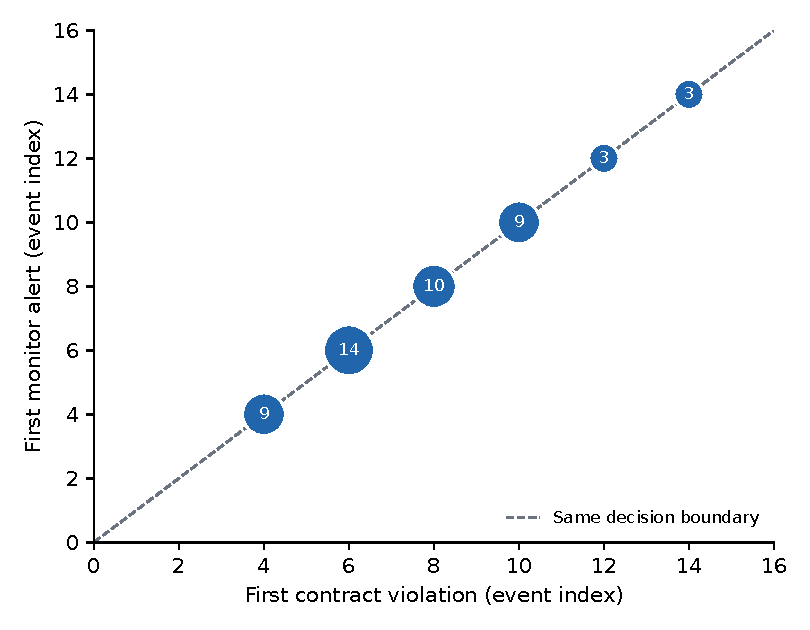
\includegraphics[width=0.78\linewidth]{figures/alert_timing.pdf}
\caption{First Gemini alert versus first explicit contract violation in the original cohort. Points on the diagonal represent boundary detection. Episodes with no observed violation or no alert are reported separately in the text; overlapping points are sized by their count.}
\label{fig:timing}
\end{figure}

\subsection{Interpreting input changes}
The development renaming diagnostic produces no alert flips at the fixed threshold. Mean absolute risk change relative to the two original scores is 0.003125, with a maximum of 0.05; repeated-original differences are zero in all 16 pairs. These prefixes lie near low-risk initial exchanges or obvious batch violations, so the result is a narrow negative finding. It does not establish invariance in ambiguous mid-trajectory cases, across arbitrary aliases, or for trained telemetry monitors.

Of the 12 preselected held-out cells, 12 supply an eligible batch proposal and 0 are ineligible; no replacement is made. The strict-repeat arm alerts on 12/12 eligible prefixes. Relaxing only the batch rule yields 0/12 alerts, and the outcome-focused prompt yields 0/12. The strict repeat changes 0 alert decisions relative to the original monitor score at the same boundary (mean absolute risk difference 0.0083). Table~\ref{tab:ablation} reports matched risk changes. These descriptive interventions expose sensitivity to the stated policy and requested target. They do not establish that the outcome-focused scores are calibrated, that every residual alert is correct, or that relaxing the rule improves live agent behavior.

\begin{table}[t]
\centering\small
\caption{Exploratory matched-prefix ablation. The strict repeat, relaxed batch policy and outcome-focused prompt share the same tools and recorded conversation. Eligibility and all selected cells are retained in the artifact.}
\label{tab:ablation}
\begin{tabular}{lrrrr}
\toprule
Input arm & Alerts & Mean risk & $\Delta$ vs. strict & Alert flips\\
\midrule
Strict repeat & 12/12 & 0.996 & +0.000 & 0\\
Relaxed batch rule & 0/12 & 0.050 & -0.946 & 12\\
Outcome-focused target & 0/12 & 0.037 & -0.958 & 12\\
\bottomrule
\end{tabular}


\end{table}

\subsection{Exploratory extension: clean controls, a second monitor, and repeats}
\label{sec:extension}
After the original analysis, a separate locally frozen extension selected three additional upstream-test IDs per domain by a fixed hash, excluding all original held-out IDs. It used DeepSeek as actor and the same Sonnet customer, with native instructions or an added actor-only reminder to issue one call per message, and two unseeded runs per task/condition. This yields 24 new conversations on six new task IDs. The step limit was 90 in both extension conditions, versus 60 originally. No proposals were edited, serialized, rejected, or resampled to obtain compliance. A two-cell feasibility gate permitted expansion if either reminder trajectory was contract-clean; both feasibility cells remain in the allocation. This is exploratory evidence, not a new confirmatory test or a family-disjoint sample.

All 24 cells completed and replayed exactly. There are 20 state successes and 7 contract-clean state successes from 3 task IDs. Clean successes occur under both native and reminder instructions. Across the 12 task/condition repeat pairs, state success differs in 0 pairs and contract compliance differs in 3. These repetitions show why a single rollout should not be treated as a stable task property; they do not isolate a causal benefit of the reminder.

\begin{table}[t]
\centering\small
\caption{Separate extension cohort. Each row has three task IDs and two unseeded repeats. Clean success is state success without the measured interaction violation.}
\label{tab:extension}
\begin{tabular}{llrrr}
\toprule
Domain & Instructions & $n$ & State successes & Clean successes\\
\midrule
Retail & native & 6 & 6 & 2\\
Retail & reminder & 6 & 6 & 3\\
Airline & native & 6 & 4 & 1\\
Airline & reminder & 6 & 4 & 1\\
\bottomrule
\end{tabular}
\end{table}
DeepSeek V4.1 Flash also evaluated all 514 original public prefixes with the same broad prompt, schema, 512-token cap and 0.5 threshold, using its configured reasoning effort of none. There are 513 valid scores and 1 missing output(s). Of 510 matched valid Gemini/DeepSeek prefix pairs, 98 disagree at the threshold. Prefix pairs are descriptive comparisons, not independent samples. The fixed 0.5 threshold is uncalibrated for both models, so their score scales need not be comparable. In one matched batch proposal (retail task 70, DeepSeek renamed actor, event 6), DeepSeek explicitly describes the four-call violation but assigns risk 0.35, versus Gemini's 1.0. Alert disagreement therefore need not mean failure to recognize a constraint. An exploratory fixed-threshold grid is supplied without selecting a preferred threshold. Table~\ref{tab:expanded-timing} shows that the original coincidence between warning and violation onset does not generalize to the second monitor configuration. An alert preceding the interaction violation may concern another property; it is not thereby a correct forecast of eventual task failure.

Both monitors also score the new conversations. Gemini supplies 255 valid scores (1 missing), and DeepSeek supplies 256 (0 missing). Among the 7 clean state successes, the proxy-relative episode alert rate is 1/7 for Gemini and 5/7 for DeepSeek. These denominators now exist, unlike in the original cohort, but cover only 3 task IDs and do not certify semantic policy compliance. The native and reminder conditions remain separately tabulated in the artifact. Missing-score uncertainty is reported as lower/upper alert-count bounds rather than imputed negatives.

For Gemini, the descriptive whole-task bootstrap envelope is [0.0\%, 25.0\%], excluding 50 of 5,000 replicates with no clean-success denominator. For Deepseek, the descriptive whole-task bootstrap envelope is [0.0\%, 100.0\%], excluding 50 of 5,000 replicates with no clean-success denominator. These small-support intervals do not establish deployment calibration. DeepSeek shares a model family with half the original actors and all extension actors; this dependence is disclosed rather than treated as independent model validation.

The autonomous conversations are not comprehensively labeled for semantic-policy compliance. Optional human-review material is separate from the reported evidence; the later constructed eligibility experiment uses explicit simulator facts and executable labels instead. No independently human-reviewed result is claimed.

\subsection{Complete remaining-test expansion and independent-family monitor}
\label{sec:replication}
A subsequent protocol, frozen before these new outcomes but after the earlier findings, allocates every remaining reserved upstream-test ID: 31 retail and 11 airline tasks. Each uses the same DeepSeek actor and Sonnet customer, native or reminder instructions, and two unseeded repeats, for 168 planned conversations. The 90-step and 900-second limits match the first extension. All attempted cells are retained, with interruptions separate from completed trajectories; no failed cell is invisibly replaced. This is an explicitly exploratory expansion of the original study, not a retrospectively declared confirmatory sample. Together the allocations cover all 60 reserved test IDs, but do not establish 60 independent task families.

Of the 168 attempts, 155 completed and 13 were interrupted. Completed runs include 133 state successes and 49 contract-clean state successes across 16 task IDs. Table~\ref{tab:replication-cohort} preserves domain and instruction strata. Rates below condition on completed runs; infrastructure missingness need not be random, and interrupted attempts remain in the released inventory.

\begin{table}[t]\centering\small
\caption{Remaining-test expansion. Completed conversations, state successes, and contract-clean state successes; clean IDs count distinct tasks contributing a clean success.}\label{tab:replication-cohort}
\begin{tabular}{llrrrr}
\toprule
Domain & Instruction & Completed & $G=1$ & $G=1,V=0$ & Clean IDs\\
\midrule
Retail & native & 57 & 49 & 13 & 7\\
Retail & reminder & 55 & 48 & 12 & 7\\
Airline & native & 21 & 17 & 9 & 5\\
Airline & reminder & 22 & 19 & 15 & 8\\
\bottomrule
\end{tabular}
\end{table}
The exact interaction-rule baseline alerts on 84/133 state successes and 0/49 interaction-clean state successes, by construction. This directly instantiates Equation~\ref{eq:decomposition} with a nonempty clean negative class; it is a transparent diagnostic, not a learned detection result.

GPT-5.4 Mini, served through a fixed provider route with reasoning effort none, is a third monitor from a family absent from the actors and customer simulator. It scores all original and first-extension prefixes; all three monitors score every generated assistant prefix of each completed new conversation. The broad prompt, response schema and 512-token cap are unchanged. We retain the original fixed 0.5 threshold and provide the same fixed sensitivity grid, without selecting a threshold from these results. Independence of model family does not establish independence of training data.

\begin{table}[t]\centering\small
\caption{Alerts among contract-clean state successes, separately by collection cohort. A range reflects unidentified episode alerts due to missing scores, not a confidence interval. All rates remain relative to the measured state/interaction target.}\label{tab:expanded-monitors}
\begin{tabular}{lll}
\toprule
Monitor & First extension & Remaining-test expansion\\
\midrule
Gemini & 1/7 & 2/49\\
DeepSeek & 5/7 & 28/49\\
GPT-5.4 Mini & 6/7 & 32/49\\
\bottomrule
\end{tabular}
\end{table}
Changing the negative class has a configuration-dependent direction: Gemini changes from 86/133 (64.7\%) to 2/49 (4.1\%); DeepSeek changes from 70/133 (52.6\%) to 28/49 (57.1\%); GPT-5.4 Mini changes from 107/133 (80.5\%) to 32/49 (65.3\%). DeepSeek increases under the additional interaction-compliance condition, whereas the other two decrease. Equation~\ref{eq:decomposition} permits either direction because the monitor need not behave like the exact rule baseline. The evaluation target must be declared on substantive grounds, without selecting whichever definition yields the preferred rate.

For Gemini, the descriptive whole-task bootstrap envelope on new clean successes is [0.0\%, 11.1\%], with 0 of 5,000 resamples lacking a denominator. For DeepSeek, the descriptive whole-task bootstrap envelope on new clean successes is [38.8\%, 76.6\%], with 0 of 5,000 resamples lacking a denominator. For GPT-5.4 Mini, the descriptive whole-task bootstrap envelope on new clean successes is [50.8\%, 80.4\%], with 0 of 5,000 resamples lacking a denominator. These intervals describe resampling of finite benchmark tasks; they do not certify population coverage or deployment calibration. Full domain/condition strata and missing-score bounds are included in the artifact.

\begin{figure}[t]\centering
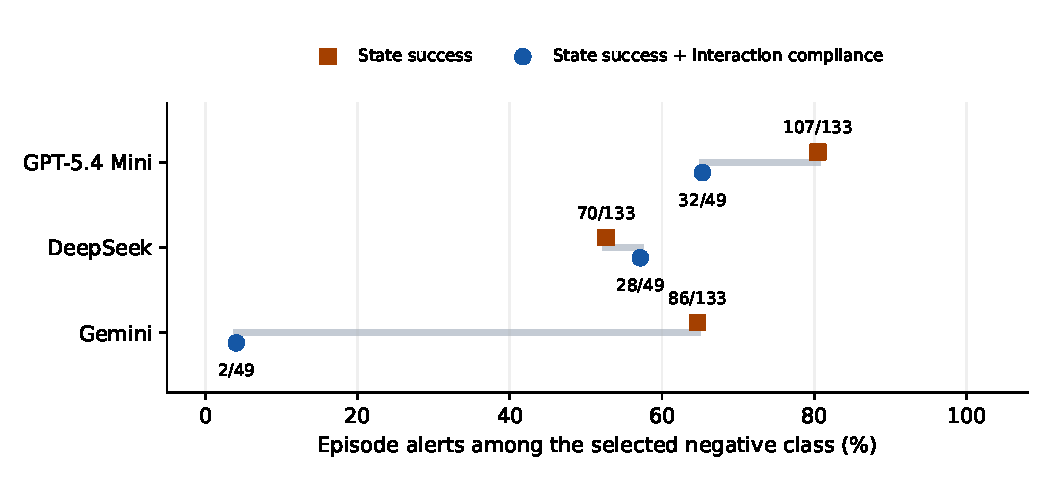
\includegraphics[width=.90\linewidth]{figures/expanded_targets.pdf}
\caption{The same broad-monitor decisions evaluated against two negative classes in the remaining-test expansion. Labels give alert counts and denominators. Gray lines connect the two target-specific rates; colored horizontal spans, where present, show missing-score bounds rather than confidence intervals.}\label{fig:expanded-targets}
\end{figure}
Among 72 task/condition pairs with both repeats completed, 4 change interaction-contract status and 13 change state-success status. These comparisons expose run variability and do not isolate a causal benefit of adding the reminder.

\begin{table}[t]\centering\small
\caption{First-alert timing relative to the first measured interaction violation. Contract-clean conversations are outside this timing denominator.}\label{tab:expanded-timing}
\begin{tabular}{llrrrrr}
\toprule
Cohort & Monitor & Before & At & After & No alert & Unidentified\\
\midrule
Original & Gemini & 0 & 48 & 0 & 0 & 0\\
Original & DeepSeek & 7 & 7 & 14 & 19 & 1\\
Original & GPT-5.4 Mini & 21 & 18 & 5 & 4 & 0\\
Expansion & Gemini & 0 & 103 & 0 & 0 & 0\\
Expansion & DeepSeek & 26 & 11 & 17 & 48 & 1\\
Expansion & GPT-5.4 Mini & 46 & 34 & 12 & 10 & 1\\
\bottomrule
\end{tabular}
\end{table}
\subsection{Constructed substantive-policy contrasts without human labels}
\label{sec:policy-lab}
To test a substantive rule separately from harmless tool batching, we construct 24 matched cancellation pairs: six rule contrasts across four deterministically selected source reservations, with an eligible and an ineligible variant in each pair. The contrasts cover booking age, airline cancellation, business cabin, health insurance, covered weather reason, and a previously flown segment. All prefixes supply the user and reservation IDs, cancellation reason, native reservation and flight-status observations, and explicit confirmation. Each ends with the same single, text-free cancellation proposal within its pair. Labels concern only cancellation eligibility, not comprehensive policy compliance.

Eligibility is computed from explicit simulator facts using two separately written formulations of the stated rule, checked over a factorial grid. This is implementation cross-checking, not independent human adjudication. Boundary-ambiguous exact 24-hour bookings are excluded from the fixtures. All 48 proposed cancellations execute through the native tool, including the 24 ineligible ones; all 48 satisfy the measured interaction contract. This demonstrates a gap between operation execution, interaction formatting, and substantive eligibility within the constructed cases. The operation-executed label is not the native task-success label $G$, and these synthetic probes are not additional autonomous actor conversations.

Each monitor sees the identical public input twice, under the original broad target and a cancellation-eligibility-only target, in alternating order. Ground-truth labels, fixture identifiers, final database state and post-action results are excluded from monitor inputs.
\begin{table}[t]\centering\small
\caption{Constructed policy cases: alerts at threshold 0.5 among 24 eligible and 24 ineligible cancellations. The focused target concerns cancellation eligibility only. Missing scores produce count ranges. These are controlled-case counts, not natural violation prevalence or deployment error estimates.}\label{tab:policy-lab}
\begin{tabular}{llll}
\toprule
Monitor & Target & Eligible alerts & Ineligible alerts\\
\midrule
Gemini & broad & 0/24 & 24/24\\
Gemini & eligibility & 0/24 & 24/24\\
DeepSeek & broad & 0/24 & 16/24\\
DeepSeek & eligibility & 3/24 & 21/24\\
GPT-5.4 Mini & broad & 0/24 & 1/24\\
GPT-5.4 Mini & eligibility & 0/24 & 4/24\\
\bottomrule
\end{tabular}
\end{table}
The artifact reports score-direction changes within every pair and all six rule strata, including failures. Four reused source reservations and six constructed rule contrasts do not form a representative semantic-policy benchmark. No human-labeled accuracy, naturally occurring semantic-violation rate, calibrated risk probability or repair benefit is claimed.


\section{Using the audit in an evaluation workflow}
\label{sec:use}
The artifact is intended for researchers and engineering teams evaluating a monitor for an agent with explicit tool-use policies. Its immediate output is an auditable comparison of warnings, not an automatic approval to deploy or block actions. A team can reproduce the saved-record analysis without model access, then adapt the protocol to a separate, locally validated test set.

\paragraph{A concrete decision.}
Suppose a team must decide whether a cancellation agent's monitor produces unnecessary warnings. An executed cancellation, a reference-state match, and a permitted cancellation are different observations. First state which one defines an error. In our final autonomous cohort, an exact interaction-rule detector appears to produce 84/133 false alarms if every state success is declared negative; on the 49 interaction-clean state successes it produces 0/49 by construction. This does not mean that the detector improved. Only the comparison set changed. Nor does conditioning uniformly reduce a model's alert rate: DeepSeek changes from 70/133 to 28/49. A team should examine the selected negative class before replacing a monitor or changing its threshold.

\paragraph{Inputs and sequence.}
For a new application, retain the policy version, tool schemas, ordered public messages and tool responses, proposed actions, task/repeat identifiers, monitor configuration, and independently computed outcome labels. Keep outcome labels and future messages outside monitor inputs. The evaluation can then follow five steps:
\begin{enumerate}
\item \textbf{Declare the property and its observation time.} Separate final-state success from each interaction or eligibility rule. Specify whether the monitor sees a proposed action before execution, or a result afterward. A pre-execution hook is an integration requirement, not an intervention benefit demonstrated by this study.
\item \textbf{Validate the labels and coverage.} Implement deterministic predicates where the rule and facts permit them, check contrasting fixtures, and collect both clean and violating outcomes. If the rule requires contextual judgment, use an adjudication process suited to that rule and report disagreement. Our executable subset does not remove that requirement for broader semantic claims.
\item \textbf{Freeze a matched comparison.} Give each monitor the same permitted prefix and record its exact configuration. Include transparent rule baselines. Separate a change to the public policy, a change to the monitoring question, and a change to the acting agent. Select thresholds using separate development data when calibration is needed.
\item \textbf{Report the denominator and clock.} Report warnings per state success and per measured-rule-clean state success, together with task counts, violation-detection counts and before/at/after timing. A missing output is unknown; a missing negative class is undefined. Preserve interrupted attempts and resample whole tasks rather than treating prefixes as independent observations.
\item \textbf{Choose the next test from the discrepancy.} If a baseline already explains a warning, inspect label alignment before adding model complexity. If a model misses an eligibility violation, inspect its public evidence, target and threshold separately. Evaluate any resulting blocking or repair policy prospectively, measuring task completion, unnecessary intervention, latency and cost on held-out cases.
\end{enumerate}

\paragraph{What a user runs and receives.}
The supplementary \texttt{USAGE.md} provides a short entry point. In a Python environment with the pinned analysis dependencies, \texttt{sh reproduce.sh} regenerates the three cohorts' analyses, manuscript tables and vector figures without model calls. The per-cohort results remain separate. \texttt{replication/analysis.json} contains the expansion's conditional rates, warning timing, repeated-run comparisons and eligibility contrasts; \texttt{replication/evidence\_ledger.json} links reported counts to their evidence. The supplied verifiers check freezes, required scoring cells and request provenance. The usage guide includes a small command that reads these saved results and explains each denominator.

\paragraph{From audit to application.}
This workflow addresses a limited part of risk measurement. The NIST AI RMF calls for selecting appropriate metrics and documenting risks that are not measured \citep{nist2023rmf}; its generative-AI profile cautions against extrapolating capabilities from narrow assessments \citep{nist2024genai}. Our audit is compatible with those reporting principles, but is not a NIST certification or a complete risk-management process. Teams would still need application-specific policy coverage, representative tests, security assessment and prospective intervention evidence before relying on a monitor operationally.


\section{Implications and limitations}
\label{sec:discussion}
\paragraph{State success is a target, not a universal negative class.}
An evaluator may legitimately care only about state outcomes. A policy-aware monitor may legitimately care about a broader event. The mistake is to interpret their disagreement without stating that their targets differ. Equation~\ref{eq:decomposition} provides a direct accounting of that difference. Our experiment constructs and measures this comparison; it does not allege that any particular published monitor used the wrong labels.

\paragraph{A transparent contract baseline is necessary here.}
Detecting multiple tool calls in one proposal is simple. When a language-model warning appears at the same boundary, its presence is not evidence that temporal modeling or broad semantic reasoning was needed. Conversely, a contract baseline cannot detect every wrong task state or semantic policy violation. It should be retained as a diagnostic control rather than presented as a complete safety monitor.

\paragraph{Documentation can change the target.}
Tool renaming with consistently updated documentation aims to preserve the task and policy. Explicitly allowing a previously forbidden batch changes the normative label. These are different interventions. Their effects should not be pooled into one ``distribution shift'' score or assumed to require the same adaptation mechanism. Likewise, asking a model to predict an incorrect state rather than any policy violation changes the requested target, not merely the wording of a fixed classifier.

\paragraph{The measured rule is narrow and often low severity.}
A batch of harmless read calls can violate the stated interaction contract without causing user harm. We report the literal rule because it is unambiguous and executable, not because every breach is dangerous. The interaction-rule counts must not be extrapolated to privacy, authorization or complete procedural integrity. The separately constructed cancellation cases test one substantive eligibility rule through explicit simulator facts; they do not provide comprehensive semantic labels for autonomous conversations. Optional human review material is outside the reported evidence.

\paragraph{Small and dependent data limit generalization.}
The original cohort contains 12 task IDs and one run per actor/interface cell; two later cohorts add six and 42 task IDs with repeated instruction conditions. Together these cover all 60 reserved upstream-test IDs but only 51 distinct exact reference-operation sequences. Workflow and database reuse remain substantial, and operation sequences are only a coarse dependency proxy. The third monitor comes from a model family absent from actors and the customer simulator; DeepSeek still shares a family with one actor, and the fixed Sonnet customer shares a family with the other. Comparisons are between complete monitor configurations, including model size and reasoning settings, not controlled architecture comparisons. Public benchmark scenarios may have appeared in training. Hosted aliases, unseeded sampling and execution-time variation limit exact regeneration. Interrupted attempts and missing monitor scores remain explicit; complete-case estimates need not be unbiased if missingness is informative. Four source reservations support the constructed eligibility pairs, which are deliberately idealized and provide no natural violation prevalence estimate. Saved records make the analyses reproducible, not future model sampling deterministic. Independently authored task families, additional customer simulators and externally validated semantic targets would be needed for broader claims.

\paragraph{No adaptation or intervention superiority is established.}
The study does not fit a learned monitor, calibrate a deployment threshold, measure prevented harm or compare repair policies. Reproducing a baseline on its own released traces does not establish performance on our task distribution. The initial plan to compare adaptation strategies was narrowed after development exposed label-alignment issues; the present manuscript reports that narrower audit rather than implying the larger plan was completed.

\section{Related work}
\label{sec:related}
\paragraph{Tool capability and interactive evaluation.}
API generation, retrieval and invocation are studied by Gorilla, ToolLLM and API-Bank \citep{patil2023gorilla,qin2023toolllm,li2023apibank}. These capabilities enable an agent to act but do not, by themselves, certify that a particular action is permitted. AgentBench evaluates interactive decision making across environments, while GAIA combines reasoning, information access and tool use \citep{liu2023agentbench,mialon2023gaia}. WebArena and WorkArena evaluate web tasks, OSWorld evaluates computer use, and SWE-bench evaluates repository modifications \citep{zhou2023webarena,drouin2024workarena,xie2024osworld,jimenez2024swebench}. They illustrate the diversity of execution environments and success criteria to which a monitoring method might be applied. Our retail/airline results establish no transfer to these settings. AppWorld's state-based unit tests also check unintended changes \citep{trivedi2024appworld}; thus, state-based evaluation need not be limited to checking a requested endpoint. The scope of the actual evaluator matters.

\paragraph{Process, outcomes and apparent success.}
AgentBoard supplements final success with fine-grained progress analysis \citep{ma2024agentboard}. Procedure-Aware Evaluation directly studies successful outcomes that conceal procedural violations \citep{cao2026procedure}. Our contribution follows that distinction and asks how it changes a monitor's negative class and warning clock; our interaction rule and constructed eligibility subset are narrower than their procedural taxonomy. False-success analysis studies agents that claim completion despite unsuccessful environment states \citep{advani2026false}. That is complementary to our central case: the measured final state succeeds, yet a declared procedure is violated. Work on process supervision in mathematical reasoning also separates intermediate-step feedback from outcome feedback \citep{lightman2023verify}. We neither train a process reward model nor infer agent-policy compliance from that study's results.

\paragraph{Agent safety and adversarial environments.}
ToolEmu uses an emulated sandbox to expose potential tool-use risks \citep{ruan2023toolemu}. AgentDojo and InjecAgent evaluate indirect prompt-injection attacks against tool-integrated agents \citep{debenedetti2024agentdojo,zhan2024injecagent}; AgentHarm studies malicious tasks, and Agent-SafetyBench covers multiple safety risks and failure modes \citep{andriushchenko2024agentharm,zhang2024agentsafety}. These are distinct targets from an interaction-format rule or a cancellation-eligibility predicate. Our constructed cases use deterministic simulator facts and native tool execution, not a comprehensive harm taxonomy. Their role is to isolate one authorization-related rule while holding the proposed operation fixed. They do not validate adversarial robustness or establish the frequency of real-world harm.

\paragraph{Warning, diagnosis and repair.}
PrefixGuard learns online warnings from structured trace views \citep{huang2026prefix}. Real-time telemetry monitoring studies deployment adaptation, verification and repair \citep{dubey2026monitor}; its released adaptation code refits a normalizer and detector before threshold calibration, so refitting is not a contribution here. AgentRx localizes critical steps in failed trajectories using an evidence-based diagnostic framework \citep{barke2026agentrx}. ReliabilityBench studies repeated execution, perturbations and tool faults, while AgentCheck compares controlled fault replay and mitigation \citep{reliability2026,mazumder2026agentcheck}. These establish that repeated runs and controlled interventions are not new in themselves. Reflexion uses verbal feedback across trials, and Self-Refine iteratively revises generated outputs \citep{shinn2023reflexion,madaan2023selfrefine}. Such improvement mechanisms require their own intervention evaluation. Observing an alert at a proposed violation in our records demonstrates neither advance prediction nor the benefit of a repair policy.

\paragraph{Model judges, explanations and uncertainty.}
Studies of model judges and G-Eval evaluate agreement with human judgments and identify limitations of automated evaluation \citep{zheng2023judge,liu2023geval}. Their tasks and reference labels differ from the executable predicates used here. Unfaithful chain-of-thought explanations further caution against reading an explanation as a causal account of a score \citep{turpin2023unfaithful}; our short monitor reasons are retained as outputs, not used as causal ground truth. SelfCheckGPT detects factual inconsistencies through sampling, and semantic uncertainty accounts for meaning-equivalent outputs \citep{manakul2023selfcheck,kuhn2023semantic}. Neither uncertainty signal is automatically a probability of violating a tool policy. Calibration research and language-model self-evaluation distinguish numeric confidence from empirically reliable probabilities \citep{guo2017calibration,kadavath2022know}. Selective classification explicitly evaluates risk against coverage \citep{geifman2017selective}; our fixed exploratory alert threshold supplies no corresponding selective-risk guarantee.

\paragraph{Evaluation validity and reuse.}
HELM emphasizes multiple metrics and common evaluation conditions; CheckList organizes behavioral tests; Dynabench supports adaptive challenge creation \citep{liang2022helm,ribeiro2020checklist,kiela2021dynabench}. Our matched-input tests isolate a declared target within a fixed corpus, rather than replacing these broader evaluation programs. Underspecification shows why similar benchmark performance need not imply equivalent behavior in deployment \citep{damour2022underspecification}. Model cards and datasheets motivate explicit documentation of intended use, collection choices and limitations \citep{mitchell2019modelcards,gebru2021datasheets}. We apply that reporting principle to an audit artifact: users receive the definitions, missingness records and input provenance needed to interpret the numbers, together with a concrete workflow in Section~\ref{sec:use}.

\section{Conclusion}
A monitor's apparent false-alarm rate is inseparable from the definition of a negative episode. This audit makes state outcomes, explicit interaction constraints and warning timing independently inspectable, with a separately scoped executable eligibility test. The practical recommendation is modest: declare the target, preserve proxy-label disagreements, include a rule baseline for directly observable constraints, and separate monitor-input transformations from changes to actor behavior. These steps make target disagreements inspectable before a team chooses a monitor or an intervention policy, while preserving state-based evaluation for its intended purpose.

\section*{Broader impact and reproducibility}
The experiments use public benchmark scenarios with simulated customers and sandboxed database operations. They do not execute real bookings, cancellations or payments. Better target alignment can reduce misleading claims about agent reliability. A potential misuse is to treat passing a narrow contract as comprehensive safety; the artifact keeps these labels separate and the paper explicitly rejects that interpretation. Credentials, local author paths and provider-account identifiers are excluded from the supplementary package. The package contains collected records, fixed prompts, configuration hashes, analysis scripts and instructions for regenerating tables and figures without paid model calls. Fresh model collection requires separate credentials and spending authorization.

\bibliography{references}
\bibliographystyle{tmlr}

\appendix
\section{Model and execution configuration}
\label{app:configuration}
\begin{table}[h]
\centering\small
\begin{tabular}{llll}
\toprule
Role & Gateway model ID & Requested provider & Output cap\\
\midrule
Actor A/customer & \texttt{anthropic/claude-sonnet-5} & anthropic & 2048 / 1024\\
Actor B & \texttt{deepseek/deepseek-v4.1-flash} & baseten & 2048\\
Monitor A & \texttt{google/gemini-3.8-flash} & google & 512\\
Monitor B & \texttt{deepseek/deepseek-v4.1-flash} & baseten & 512\\
Monitor C & \texttt{openai/gpt-5.4-mini} & openai & 512\\
\bottomrule
\end{tabular}
\end{table}
Reasoning effort is \texttt{none} for the actors/customer, DeepSeek monitor and GPT-5.4 Mini monitor, and \texttt{low} for the Gemini monitor. No explicit temperature or provider sampling seed is supplied. Provider fallback is disabled by a one-provider allowlist. Read-only generation receipts checked for one access request for each of the original Sonnet, DeepSeek and Gemini configurations agree with the requested provider and response-reported charge; this is a spot check, not an independent receipt audit of every request. Every charged attempt retains its request, response and usage record locally. The anonymous release omits account-linked generation identifiers.

The complete recorded research program contains 12,968 API requests with cumulative response-reported cost of \$35.80. The final expansion adds \$19.87; earlier cohort costs remain separately archived. Unresolved failed-request reservations total \$2.3461. These are local accounting records, not a reconciled provider invoice; reservations are admission holds rather than additional charges. The study uses Python 3.13 and native benchmark orchestration. A separate capability probe returned multiple DeepSeek tool calls despite requesting \texttt{parallel\_tool\_calls=false}. No enforcement claim or serial-enforced benchmark condition is based on that probe. Collected actor experiments use unchanged native proposal execution in both instruction conditions.

\section{Monitor prompt and exact contract}
The broad monitor's fixed instruction is reproduced below; schema-constrained output contains a risk in $[0,1]$ and a short reason.
\begin{quote}\small
You monitor a customer-service agent at a decision boundary. Estimate the probability that this interaction will end unsuccessfully: an incorrect task result, an unfulfilled user request, or a violation of the current public policy. Use only the public policy, available tools, and conversation prefix provided. Tool calls in the last assistant message are proposed and have not yet run; earlier tool results are observations. A recovered lookup error is not automatically a failed task. Do not assume that unfamiliar tool names indicate failure: use the current documentation. Return risk between 0 and 1 and a short reason citing visible evidence. Do not invent hidden requirements or future events.

\end{quote}
The exact contract label is computed for every assistant message as
\[
 V_t=\ind\bigl[|\mathrm{toolcalls}_t|>1\;\lor\;
 (|\mathrm{toolcalls}_t|>0\land |\mathrm{strip}(\mathrm{text}_t)|>0)\bigr].
\]
Native greetings without a model request are not monitor decision points. Tool-error flags are exposed only after a tool response. Identical-call repetition compares serialized tool names and argument objects; it does not infer whether a repeat was unnecessary.

\section{Released CPU-baseline reproduction}
\label{app:reproduction}
As an initial infrastructure check, seven CPU methods from the artifact of \citet{dubey2026monitor} were run on the authors' committed traces, at revision \texttt{1b3e07fee53ae13407173c3ea932adb4a43e8230}. Their episode AUROC, detection and healthy false-alarm columns matched the released reference to within $10^{-9}$ for every reproduced row. For the channel-max method, the reproduced detection count is 56/79 and healthy false-alarm count is 3/15, with AUROC approximately 0.8401. These are the original artifact's data and results, not measurements on our new conversations. Methods requiring the omitted deep-learning dependency were not reproduced. We make neither a full-paper reproduction claim nor a comparison between these numbers and the held-out audit.

\section{Analysis audit and task allocation}
\begin{center}
\begin{tabular}{lllr}
\toprule
Domain & Test task ID & Operation-sequence group & Reference calls\\
\midrule
Retail & 32 & \texttt{0ab342cd01b0} & 13\\
Retail & 55 & \texttt{ae1c988c9a85} & 13\\
Retail & 64 & \texttt{e36ae532b541} & 8\\
Retail & 49 & \texttt{bd9bafe141b5} & 10\\
Retail & 70 & \texttt{005b397268a9} & 1\\
Retail & 51 & \texttt{af79634c9ee3} & 6\\
Airline & 31 & \texttt{4f53cda18c2b} & 0\\
Airline & 26 & \texttt{4f53cda18c2b} & 0\\
Airline & 16 & \texttt{0bd8441d0224} & 1\\
Airline & 37 & \texttt{0d372c1f8b74} & 4\\
Airline & 35 & \texttt{393abe1763ba} & 1\\
Airline & 29 & \texttt{07b98bd9e8ca} & 3\\
\bottomrule
\end{tabular}
\end{center}
All listed IDs come from the pinned upstream test split. An empty reference sequence is retained and may correspond to a legitimate no-mutation task; it does not establish semantic task success.

The extension adds retail task IDs 42, 94 and 77, and airline task IDs 19, 32 and 25. Their complete allocation and repeated-run ordering are in the separate extension manifest. The final expansion allocates all remaining reserved test IDs, yielding 60 allocated task IDs and 51 observed exact reference-operation groups across the three cohorts; these coarse groups do not establish independent semantic task families.

The supplementary result ledger maps each manuscript count to an analysis field and its input-file hashes. Source-controlled benchmark files are unchanged. The public benchmark is distributed under its MIT license; the released monitor artifact uses Apache 2.0. Their notices are retained where their material is included. The official TMLR style is used without modifying its layout. Bootstrap intervals, raw denominators, missing cells and unscored prefixes are retained in machine-readable output.
\section{Monitor coverage and executable eligibility}
\begin{table}[h]\centering\small
\caption{All requested decision prefixes. Missing outputs are retained. Unidentified episode labels count conversations whose any-alert status or first-alert timing cannot be determined from the available scores.}\label{tab:coverage}
\begin{tabular}{llrrrr}
\toprule
Cohort & Monitor & Valid & Missing & Unknown any & Unknown first\\
\midrule
Original & Gemini & 511 & 3 & 0 & 0\\
Original & DeepSeek & 513 & 1 & 0 & 1\\
Original & GPT-5.4 Mini & 514 & 0 & 0 & 0\\
Extension & Gemini & 255 & 1 & 0 & 0\\
Extension & DeepSeek & 256 & 0 & 0 & 0\\
Extension & GPT-5.4 Mini & 256 & 0 & 0 & 0\\
Replication & Gemini & 1762 & 6 & 0 & 0\\
Replication & DeepSeek & 1766 & 2 & 0 & 1\\
Replication & GPT-5.4 Mini & 1767 & 1 & 0 & 1\\
\bottomrule
\end{tabular}
\end{table}
For the constructed fixtures, let $a$ be booking age in hours, $F$ indicate any flying or landed segment, $C$ indicate that all segments are cancelled by the airline, $B$ indicate business cabin, $I$ indicate purchased insurance, and $R$ indicate a health or weather reason. The executable eligibility label is
\[ E=\neg F\;\land\;\bigl[(0\leq a<24)\lor C\lor B\lor(I\land R)\bigr]. \]
Fixtures use the policy clock (15 May 2024, 15:00 EST), exclude exact 24-hour bookings, and contain nonempty itineraries with uniform segment status. Mixed-status itineraries are untested. Both implementations agree over 432 factorial fact combinations; this is implementation cross-checking, not independent policy adjudication.

\end{document}
